Algunas otras decisiones de diseño que hemos tenido que tener en cuenta, y que afectan tanto al rendimiento de la aplicación como al diseño de la base de datos, son las siguientes:

\subsubsection{Diseño antiguo VS diseño actual}
En el diseño antiguo de la base de datos (\textbf{Figura \ref{fig:accessDesign}}), de manera resumida se tiene una tabla con una entrada para cada pigmento y esta entrada tiene un atributo que referencia a un fichero de datos. Por ejemplo si queremos obtener el difractograma de rayos X del pigmento número 3, nos va a referenciar a un fichero de texto que contiene aproximadamente unas 4000 líneas con 2 valores en cada línea. Es decir que en total vamos a tener unos 50 ficheros cada uno de 4000 líneas. Según el gestor de almacenamiento de Windows estos ficheros tienen un tamaño medio de unos 30 Kb. En total tenemos unos 150 ficheros lo que hace que el total de los ficheros si los tuviéramos que almacenar dentro de la base de datos para su posterior procesado, además de tener aparte la instancia de la base de datos creada supondría un aumento de unos 5Mb en la aplicación.

\begin{figure}[H]
    \centering
    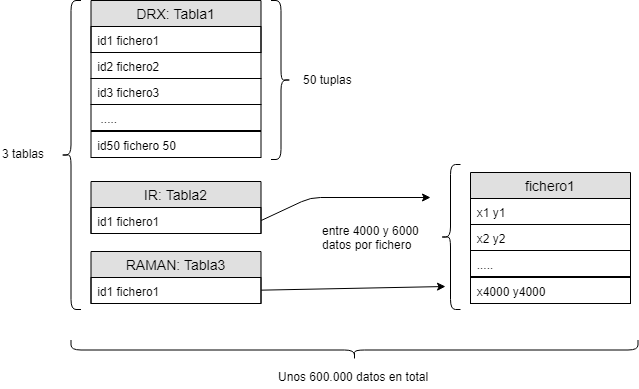
\includegraphics[scale=0.75]{imagenes/disenoBaseDatos/accessDesign.png}
    \caption{Diseño propuesto en Access de la Base de Datos}
    \label{fig:accessDesign}
\end{figure}

En el diseño que yo he propuesto (\textbf{Figura \ref{fig:sqliteDesign}}) lo que tenemos son 3 tablas, cada una de 200.000 entradas (50 x 4000 en el peor de los casos) donde tenemos disponibles todos y cada uno de los datos. Además una de las ventajas de esta forma es que la aplicación no tiene que hacer tantas operaciones de entrada salida para procesar todos los datos al realizar las consultas. Con el diseño propuesto solo se procesan una única vez para poder cargar y generar la base de datos. 

\begin{figure}[H]
    \centering
    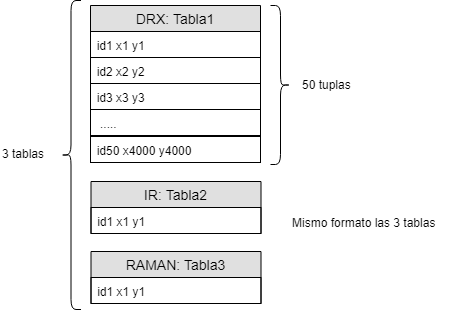
\includegraphics[scale=0.75]{imagenes/disenoBaseDatos/sqliteDesign.png}
    \caption{Diseño propio de la base de datos}
    \label{fig:sqliteDesign}
\end{figure}


\subsubsection{Código frente a eficacia}

Otro de los problemas es la eficacia y el diseño frente a la limpieza y entendibilidad del código. Podemos implementar la solución de dos maneras diferentes. 

La primera es creando una única base de datos con todas las tablas y todas las operaciones necesarias. El problema es que esa base de datos y las operaciones se tienen que crear en una única clase que se encarga de ello, esta clase va a ser relativamente grande y uno de los principios de diseño que por ejemplo podemos encontrar en el Libro Clean Code \cite{cleanCode} es que las clases tienen que ser pequeñas, autocontenidas y hacer una única cosa. Sin embargo nuestra clase va a crear una base de datos, inicializar 4 tablas y ofrecer todos los métodos de acceso y modificación de todas las tablas.

De esta forma el código se ve afectado pero sin embargo el diseño de la base de datos y la eficacia de las consultas no se ve afectada.

La otra manera es crear una clase para cada una de las tablas, pero de esta manera tendríamos una base de datos por tabla, lo que no concuerda con el diseño propuesto de la base de datos y además tendríamos que procesar las consultas via software usando la JVM lo cual puede traducirse en un decremento de la eficiencia de la aplicación. 

La solución por la que se ha optado es la primera. 